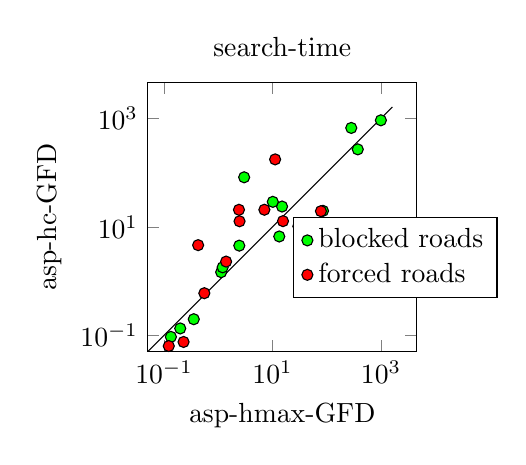
\begin{tikzpicture}
\begin{axis}[extra x tick style={grid=major}, extra x ticks=10000, extra y tick style={grid=major}, extra y ticks=10000, height=5cm, legend cell align=left, legend style={at={(1.3, 0.5)}}, title=search-time, width=5cm, xlabel=asp-hmax-GFD, xmin=0.05, xmode=log, ylabel=asp-hc-GFD, ymin=0.05, ymode=log]
\addplot[color=green, mark=*, mark options={{draw=black}}, only marks] coordinates {
(3.000890, 81.811600) (1.131580, 1.458470) (0.134073, 0.093680) (0.353865, 0.198306) (85.232500, 19.691200) (14.997400, 23.659700) (0.112922, 0.016453) (993.857000, 918.556000) (2.442110, 4.498780) (372.842000, 267.636000) (13.319200, 6.637240) (10.123400, 28.868500) (1.205280, 1.793270) (0.199281, 0.133952) (282.845000, 664.828000)
};
\addlegendentry{blocked roads}
\addplot[color=red, mark=*, mark options={{draw=black}}, only marks] coordinates {
(0.122506, 0.063470) (11.175300, 174.963000) (15.600200, 12.727900) (1.395690, 2.286330) (0.554129, 0.597915) (0.425890, 4.595660) (2.408420, 20.600400) (0.229445, 0.075522) (7.084070, 20.647500) (29.961400, 10.242900) (78.106600, 19.433000) (2.468450, 12.658600)
};
\addlegendentry{forced roads}
\addplot[color=black] coordinates {(0.050000, 0.050000) (1618, 1618)};
\end{axis}
\end{tikzpicture}
